\chapter{Grundlagen}%

\label{cha:Schluss}

In dieser Arbeit werden einige Technologien genutzt um die Problemstellung zu lösen.
Die wichtigsten dieser Technologien werden hier erklärt, um das weitere Verständniss des Lesers zu gewährleisten. 


\section{Vier Gewinnt}
Vier Gewinnt ist ein Spiel für 2 Spieler in dem abwechselnd Spielsteine in ein vertikales Spielfeld der größe 7 * 6 eingeworfen werden. Jeder Spieler kann sich in seinem Zug zwischen einem von sieben Einwurflöchern entscheiden. Wird ein Spielstein eingeworfen so fällt dieser auf die niedrigste der sechs Positionen die noch nicht durch andere Spielsteine gefüllt ist. Hierdurch ergibt sich ein Spielfeld mit 42 Feldern.  Sind schon sechs Spielsteine in ein bestimmtest Einwurfloch gesteckt wurden so darf hier kein weiterer Spielstein eingeworfen werden. Ein Spieler gewinnt das Spiel wenn er es geschafft  hat, dass sich vier seiner Spielsteine in einer Reihe befinden. Eine Reihe kann horizontal, vertikal oder diagonal gebildet werden. Werden alle 42 Positionen mit Spielsteinen befüllt ohne eine Reihe von vier Steinen des selben Spielers zu bilden geht die Partie unentschieden aus.
\begin{figure}[h!]
  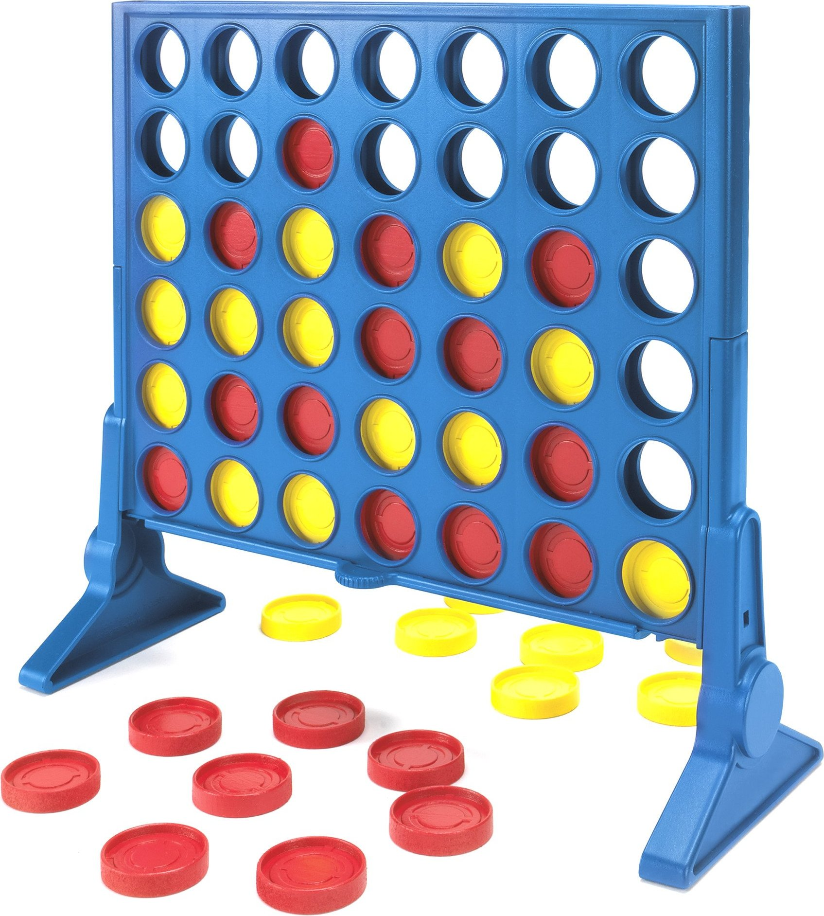
\includegraphics[scale=0.1]{echtes_spiel.png}
  \centering
  \caption{Das Spiel Vier Gewinnt}
  \label{fig:echtes_spiel}
\end{figure}


\section{Minimax Algorithmus}
Ein Minimax Algorithmus beschreibt einen rekursiven Ansatz zum Finden einer optimalen Lösung für Probleme von zwei Parteien mit widersetzlich Zielen. Dies sind in der Regel Nullsummenspiele mit perfekter Information, es gibt also für jeden Gewinn des einen Spielers genauso viel Verlust für den anderen und es gibt kein Spielelement, dass nur für einen Spieler einsehbar ist. Der Minimax Algorithmus berechnet sich hierfür den Suchbaum des Spiels, welcher alle möglichen Züge beider Spieler in nachvollziehbarer Reihenfolge enthält. Hierbei werden in jedem Rekursionsschritt alle möglichen Züge des derzeitigen Spielers betrachtet und bewertet. Wenn der derzeitige Zug nicht zum Gewinn führt, findet eine Bewertung durch das Betrachten des nächsten Rekursionsschrittes statt. 
Der Name Minimax ergibt sich durch das Betrachten der abwechselnden besten Züge von den Spielern. Da dies aus der Perspektive von einem Spieler betrachtet wird, ergibt sich hieraus ein abwechselnd minimaler und maximaler Zug. Dieses Verfahren führt bei einfachen Spielen wie Tic-Tac-Toe zu einem perfekten Spieler, da hier eine überschaubare Menge an möglichen Zügen betrachtet wird (9 Felder die von 2 Spielern gefüllt werden). Für komplexere Probleme gibt es die Möglichkeit eine Suchtiefe zu bestimmen, wodurch die Rekursion  nur bis zu dieser Tiefe durchgeführt wird. Dies ist Sinnvoll da die Berechnung einzelner Züge sonst sehr lange dauern kann. Der Minimax Algorithmus kann in bestimmten Spielen noch verbessert werden. Diese Verbesserungen sind der Negamax Algorithmus und die Alpha-Beta Suche welche im Folgenden einmal beschrieben werden.  Der Einfachheit halber wird trotz dieser Erweiterungen in dieser Arbeit im Bezug auf diesen Algorithmus immer von Minimax geredet.

\subsection{Negamax Algorithmus}
Der Negamax Algorithmus basiert auf der Annahme, dass der maximal beste Zug für den einen Spieler der minimal beste Zug für den anderen bedeutet. Ist dies so in einem Spiel in dem beide Spieler in jedem Zug die selben Dinge tun können, kann hierdurch die Rekursion vereinfacht werden, indem für beide Spieler die selbe Formel benutzt wird. Hierfür muss dann in jedem Rekursionsschritt der Input negiert werden. Wegen dieser Negierung heißt dieser Algorithmus auch Negamax.

\subsection{Alpha-Beta Suche}
Alpha-Beta Suche ist eine Variante des Minimax Algorithmus, die die Berechnung des Suchbaumes beschleunigt, indem sie bestimmte Teile der Suche nicht ausführt wenn es schon einen klar besseren Pfad gibt.

\section{Reinforcement Learning}
Reinforcement learning (Bestärkendes Lernen) ist eine Maschine-Learning Methode bei der ein Agent mit Hilfe eines Environments, Policy, State, Actions und eines Rewards lernt, eine ihm gegebene Aufgabe zu lösen. Es wird dabei Grundsätzlich wie in Abbildung \ref{fig:rl_basic} beschrieben vorgegangen. Der Agent bekommt also einen State vom Environment, und durch diesen sucht  er sich mittels seiner Policy eine Action aus. Diese Action beinflusst dann das Environment und dieses gibt dem Agenten einen Reward für seine Action. Durch den Reward kann der Agent dann seine Policy anpassen. Dazu bekommt der Agent dann den neuen State und kann dann, mit der angepassten Policy, wieder eine neue Action auswählen. Diese Teile des reinfocement learnings werden hier nun einmal genauer beschrieben.\\

\begin{figure}[h!]
  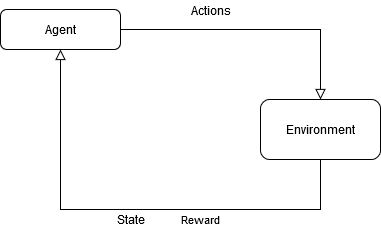
\includegraphics[scale=0.5]{rl_basics.png}
  \centering
  \caption{grundsätzliches Konzept von reinforcement learning}
  \label{fig:rl_basic}
\end{figure}

\subsection{Environment}
Das Environment beschreibt das gesamte Problem dass der Agent versucht zu lösen. Es beinhaltet alles was für das Spielen wichtig ist außer dem Spieler, welcher von dem Agenten behandelt wird.  Dies ist bei den meisten Spielen ein Spielfeld mit den Positionen aller Akteure, Spielsteine oder sonstige Elemente die zum Spielen genutzt werden. Dazu kümmert sich das Environment auch noch um die Spiellogik. Die Spiellogik beschreibt alle Abläufe die durch die Regeln des Spiels definiert wurden. In dem Beispiel Vier Gewinnt wäre das unter anderem die Funktion, dass die Spielsteine immer auf das untereste freie Feld fallen oder die Überprüfung ob ein Spieler gewonnen hat. Das letzte wichtige Element im Environment der meisten Spiele ist der Gegenspieler welcher im Falle von physikalischen Spielen normalerweise die selben Möglichkeiten besitzt wie der Spieler. Für das Verhalten des Gegenspielers werden im Normalfall Algorithmen genutzt die den bestmöglichen Zug errechnen, wie hier der Minimax Algorithmus. Für sehr komplexe Spiele bei denen sich kein optimalerZug berechnen lässt wird oft auf menschliche Spieler zurückgegriffen. Da ein Computer aber viel schneller im spielen ist und reinforcement learning viele Durchläufe absolvieren muss um Wirkung zu zeigen wird versucht dies zu vermeiden oder bestehende Datensätze von Spielen mit Menschen genutzt.\\


\subsection{Agent}
Bei dem Agenten handelt es sich um den Akteur der die ihm gegebene Aufgabe meistern soll. Er sieht das Environment und wählt mittels der Policy die ihm am besten erscheinende Action aus um den Reward zu maximieren.\\

\subsection{Policy}
Mit der Policy wird das Verhalten beschrieben nach dem der Agent entscheidet welche der möglichen Aktionen die aktuell beste ist um den Reward zu maximieren.\\
\colorbox{red!30}{TODO} %welche gibt es so?

\subsection{State}
Der State beschreibt den aktuellen Zustand des Environments welcher in jedem Zug  an den Agenten weitergereicht wird, damit dieser seine Auswahl treffen kann. 

\subsection{Actions}
Actions sind die möglichen Aktionen zwischen denen sich der Agent je nach State entscheiden muss. Diese sind alle möglichen Züge die ein Spieler zu einer bestimmten Zeitpunkt ausführen kann.

\subsection{Reward}
Der Reward ist die Belohnung die der Agent für seine Aktionen bekommt. Diese Belohnung beschreibt, wie gut es ist eine bestimmte Aktion auszuführen. Hieran passt der Agent dann wärend des Trainings seine Q-Values entsprechend seiner Policy an. Der Reward wird also benutzt um das Verhalten des Agenten zu beeinflussen. Möchte man ein bestimmtes Verhalten wird hierfür ein positiver Reward vergeben. Möchte man ein anderes Verhalten nicht wird ein negativer Reward vergeben. Je besser die  Reward-Funktion gewählt wird desto eher wird der Agent gewolltes Verhalten zeigen. Bei der Wahl einer Reward-Funktion wird zwischen diskreten und  kontinuierlichen Funktionen unterschieden, es ist aber auch eine Mischung dieser beiden möglich.\\
Bei einer diskreten Reward-Funktion werden nur feste im vorhinein definierte Rewards gegeben die zu bestimmten Events verteilt werden. Solch ein Event kann zum Beispiel das Gewinnen und Verlieren am Ende eines Spiels sein oder das Betreten des Agenten in einen gewollten oder ungewollten Bereich. \\
Bei einer kontinuierlichen Reward-Funktion wird der Reward zu jedem Schritt durch verschiedene Faktoren aus dem Environment berechnet. Solche Faktoren können zum Beispiel die verstrichene Zeit oder die Anzahl der Züge oder die aktuelle Position des Agenten sein. Eine gute kontinuierliche Reward-Funktion hilft dabei den Agenten schneller dem gewünschten Verhalten anzunähern indem der Reward zu den gewünschten Zielstates hin immer weiter angehoben wird.\\ 
Da diese beiden Arten von Reward-Funktionen das Verhalten des Agenten an unterschiedlichen Stellen beeinflussen, ist es oft sinnvoll eine Mischung dieser zu nutzen.
Wird sich für eine Mischung entschieden ist es wichtig, dass die aus beiden Teilen kommenden Rewards in Relation zueinander stehen, denn sonst kann dies dazu führen, dass die Auswirkung von dem Teil mit kleineren Rewards von dem Teil mit größeren Rewards überschattet wird.\\

Bei Komplexeren Environments ist es schwer für jeden Zug vorauszusehen wie Zielführend er ist. Um diesem credit assignment problem entgegen zu wirken wird Q-Learning genutzt.
Deswegen wird hier dann eine Q-Funktion benutzt die anhand der gelernten Zustände versucht Fehlende zu Approximieren.\colorbox{red!30}{TODO}

\subsection{Q-Funktion}
\colorbox{red!30}{TODO} %ausführen

\subsection{Q-Values}
\colorbox{red!30}{TODO} %ausführen

\subsection{Markov Decision Process}
\colorbox{red!30}{TODO} %ausführen

\subsection{Deep Q-Network}
Da es, bei einem Spiel mit einer Komplexität wie Vier Gewinnt, nicht möglich ist für alle Paare von State und Action einen erwarteten Reward zu bestimmen, wird ein neuronales Netz genutzt welches versucht eine Policy für diese erwarteten Rewards zu bestimmen. Dieses Verfahren nennt sich Deep Q-Learning. Hierbei wird ein Deep Q-Network erstellt, welches durch eine Sammlung zufälligen gespeicherter Spielen mit der aktuellen Policy diese anpasst.
\colorbox{red!30}{TODO} %ausführen

\subsection{Episode}
Eine Episode beschreibt einen einzelnen Durchlauf des Agenten im Environment.

\subsection{Epoche}
Eine Epoche ist eine Sammlung von Episoden und beschreibt einen gesammten Lerndurchlauf.


%\colorbox{red!30}{TODO Beispiele} %ausführen






\section{Software}
Um die Problemstellung zu bearbeiten wurde eine Implementierung des Spiels in Python genutzt welches als ein OpenAI Gym Environment fungiert. An diesem Environment trainiert dann ein Agenten der mit Hilfe von  Keras erschaffen wurde.
\colorbox{red!30}{TODO genaue versionen}

\subsection{Python}
Als Programmiersprache wurde sich für Python entschieden da ein gutes Vorwissen in dieser Sprache vorhanden war und alle für diese Arbeit wichtigen Packages in dieser Programmiersprache existieren.
Der Schöpfer von Python beschreibt es selbst als einfach zu erlernende objektorientierte Programmiersprache, welche Leistung mit einer klaren Syntax verbindet.\\
\colorbox{red!30}{TODO https://dl.acm.org/doi/book/10.5555/1593511}

\subsection{Tensorflow}
Bei Tensorflow handelt es sich um ein open source Framework für Maschine-Learning welches ursprünglich für den internen Bedarf bei Google, für zum Beispiel Spracherkennung oder Google Maps, entwickelt wurde. 

\subsection{Keras}
Keras ist eine open source Bibliothek die auf Tensorflow aufbaut welche die Möglichkeit bietet vereinfacht neuronale Netze zu erstellen um diese in reinforcement learning Algorithmen zu benutzen.

\subsection{OpenAI Gym}
Gym \cite{gym} ist ein Werkzeug zum Entwickeln und Vergleichen von reinforcement learning Algorithmen welches von OpenAI, einem Forschungslabor aus San Francisco, zur Verfügung gestellt wird. Es bietet einen Standard zwischen dem Environment und dem Agenten. Hierdurch können neue Agenten und Environments nach gewissen Vorgaben erstellt werden. Somit ist es mit Gym einfacher möglich verschiedene Agenten an einem Environment zu Trainieren und diese zu vergleichen oder den selben Agenten an verschiedenen Environments auf seine Anpassungsfähigkeit zu testen.

